\documentclass{article}


% if you need to pass options to natbib, use, e.g.:
%     \PassOptionsToPackage{numbers, compress}{natbib}
% before loading neurips_2024


% ready for submission
\usepackage{neurips_2024}


% to compile a preprint version, e.g., for submission to arXiv, add add the
% [preprint] option:
%     \usepackage[preprint]{neurips_2024}


% to compile a camera-ready version, add the [final] option, e.g.:
%     \usepackage[final]{neurips_2024}


% to avoid loading the natbib package, add option nonatbib:
%    \usepackage[nonatbib]{neurips_2024}


\usepackage[utf8]{inputenc} % allow utf-8 input
\usepackage[T1]{fontenc}    % use 8-bit T1 fonts
\usepackage{hyperref}       % hyperlinks
\usepackage{url}            % simple URL typesetting
\usepackage{booktabs}       % professional-quality tables
\usepackage{amsfonts}       % blackboard math symbols
\usepackage{nicefrac}       % compact symbols for 1/2, etc.
\usepackage{microtype}      % microtypography
\usepackage{xcolor}         % colors

\usepackage{orcidlink}
\usepackage{graphicx}
\usepackage{amsmath}
\usepackage{amssymb}
\usepackage{booktabs}
\usepackage{algorithm}
\usepackage{algpseudocode}
\usepackage{graphicx}
\usepackage{booktabs}

% Define the title
\title{Communication-Efficient \& Class-Balancing Federated Learning with Adaptive Dropout \& Model Quantization}

% Define the author(s)
\author{%
  Shaif Chowdhury \\
  Computer Science Department\\
  Baylor University\\
  \texttt{Shaif_chowdhury1@baylor.edu} \\
  \And
  Aaron Carney \\
  Computer Science Department\\
  Baylor University\\
  \texttt{Aaron_carney1@baylor.edu} \\
}

\begin{document}
\maketitle


% The \author macro works with any number of authors. There are two commands
% used to separate the names and addresses of multiple authors: \And and \AND.
%
% Using \And between authors leaves it to LaTeX to determine where to break the
% lines. Using \AND forces a line break at that point. So, if LaTeX puts 3 of 4
% authors names on the first line, and the last on the second line, try using
% \AND instead of \And before the third author name.


\begin{abstract}

Federated learning(FL) is used to train deep learning models over over heterogeneous and decentralized datasets. Communication between client and server can be a major bottleneck for Federated learning, specially in case of large models. More over there is often data imbalance issue in real world FL problems. 

To address the above mentioned issues we propose a novel balanced communication efficient federated learning strategy. Our strategy is based on two key strategies : 1. A novel Adaptive federated dropout on client models to address both communication bottleneck and data imbalance. 2. Quantization method to improve communication efficiency. We empirically show that the combination of these two strategies improve communication strategy while improving the accuracy of the model on several data set and experimental settings. The code can be found at anonymous.

\end{abstract}

\section{Introduction}

\subsection{Motivation for Federated Learning}

The digital era is witnessing an unprecedented increase in data generation, much of which is highly sensitive and personal. This surge necessitates the advancement of deep learning models that can be trained over decentralized and heterogeneous datasets, thus ushering in the era of federated learning (FL). FL represents a paradigm shift from traditional centralized machine learning approaches by enabling the training of models directly on devices where the data is generated \cite{info13050263}. This method ensures data privacy since the raw data never leaves its original device, thereby addressing growing concerns over data security and privacy in the age of information\cite{mao2022communication, zhang2022homomorphic}.\par

The cornerstone of FL lies in its ability to maintain the confidentiality and integrity of data. In traditional machine learning approaches, data aggregation poses significant risks of privacy breaches. However, FL aims to circumvent this issue by decentralizing the data processing, thereby safeguarding sensitive information. This approach can not only enhances user trust but also complies with stringent data protection regulations such as the General Data Protection Regulation (GDPR)\cite{team2020eu} in Europe .\par

While FL presents an innovative solution to privacy concerns, it introduces unique challenges stemming from the decentralized nature of data. These challenges include managing data heterogeneity across different devices and ensuring model performance despite the varying quality and quantity of local datasets. The decentralized framework of federated learning necessitates novel approaches to model training and aggregation to tackle these obstacles efficiently while maintaining the aforementioned privacy tenets.\par

\subsection{Challenges in Federated Learning}

\subsubsection{Communication Bottleneck}
One of the paramount challenges in FL is the communication bottleneck that arises, especially with large deep learning models. The necessity to frequently exchange model updates between the server and numerous clients can lead to significant communication overhead \cite{nader2020adaptive}. This issue is exacerbated in scenarios with limited bandwidth or when the model size becomes substantially large, thereby straining network resources and impacting the efficiency of the learning process.\par

\subsubsection{Data Imbalance}
Another significant challenge is the inherent data imbalance across clients in FL settings. Given that data is generated in a non-IID (independent and identically distributed) manner across different devices, some clients may have more data or more diverse data than others. This imbalance can lead to skewed model updates, where the model disproportionately learns from clients with more or more varied data, potentially compromising the overall model performance and fairness \cite{10.1093/comjnl/bxac118, jeon2024federated}.\par

\subsubsection{Proposed Solution}

Neural Network quantization techniques can play a critical role in mitigating communication bottlenecks. While regularization methods like dropout can improve model performance as well as improve communication efficiency \cite{srivastava2014dropout}. Dropout works by  randomly "dropping out" (setting to zero) a certain percentage of neural network units during the training. When combined with an appropriate quantization method dropout can significantly reduce the amount of data transmission between client and server. Such reduction is vital for the efficient transmission of model updates over networks with limited bandwidth \cite{10472332}. Furthermore, incorporating dropout can also serve as an effective regularization technique. It improves model robustness against over-fitting and enhances its generalization capabilities across decentralized datasets \cite{srivastava2014dropout,DBLP:journals/corr/abs-2109-15258}.\par

Furthermore, the application of dropout and quantization techniques can inadvertently bolster the security of federated learning systems. By reducing the model's complexity, the potential attack surface for adversarial attacks is minimized, thereby safeguarding both the integrity of the model and the privacy of user data \cite{TANG2024269}. This dual benefit underscores the importance of model compression not only for improving FL efficiency and scalability but also for reinforcing the security posture of federated learning ecosystems against evolving cyber-security threats.\par

\begin{figure*}
  \centering
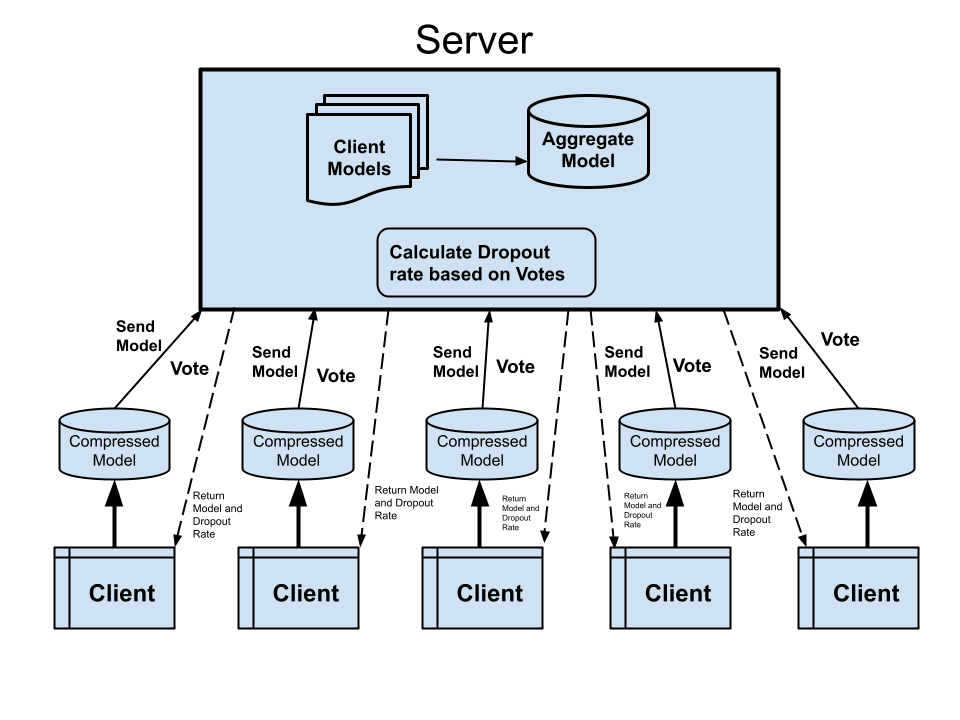
\includegraphics[width = \linewidth, height = .55\linewidth]{img/1.Fed_Lr.png}
\caption{A block diagram of Adaptive Federated learning with Quantization.}
  \label{fig:fed_lr}
\end{figure*}

In this paper, we propose two novel strategies to mitigate the communication footprint in federated learning and provide empirical evidence demonstrating that our model is robust to data imbalance. The specific contributions of this study are as follows:

\textbf{Adaptive Federated Dropout} innovates by integrating the conventional Dropout \cite{srivastava2014dropout} technique, previously proposed federated dropout \cite{wen2022federated, caldas2018expanding} with and a voting based adaptive dropout method inspired by CLIMB Algorithm \cite{shen2021agnostic}. Our method involves training client models that start with a fixed dropout rate, but adjust this rate dynamically based on model performance feedback from the server. The clients vote to either increase or decrease the dropout and based on that server makes a decision. If a client model achieves higher accuracy than what the server model returns, then it votes to increase the dropout rate; conversely, it votes to decrease if the server's model performs better.\par

\textbf{Model Quantization} forms our second approach to reducing the communication footprint in federated learning environments significantly. By implementing various quantization levels introduced before \cite{jacob2018quantization}, from float16 to int8, this method efficiently lowers bandwidth requirements while negligibly affecting model performance. Our experiments across multiple benchmark datasets showcase the robustness of model quantization, particularly when combined with adaptive dropout techniques, even on datasets with class imbalances like imbalanced-cifar.\par

\textbf{Empirical Validation} through experiments on several benchmark datasets confirms the effectiveness of our proposed strategies. The combined use of adaptive dropout and model quantization not only conserves bandwidth but also proves robust against class imbalances, thereby providing a compelling case for their application in practical federated learning scenarios. We also provide our source-code with examples to make it easy to integrate our method with existing federated learning frameworks and different model architectures.\par

\section{Related Work}

\subsection{Foundations of Federated Learning} 
Federated learning (FL) has emerged as a paradigm that leverages vast, dispersed datasets while ensuring privacy protection. Originating from the work of McMahan et al.\cite{DBLP:journals/corr/McMahanMRA16} in 2016, FL enables model training across multiple devices without centralizing data, thus addressing the privacy and security limitations of traditional cloud-based methods. By decentralizing the process, FL enhances privacy and reduces the bandwidth needed for data transfer, a significant advantage in the era of rapid digital expansion \cite{ijerph20156539}.

At the core of FL are principles of collaborative model training. Data remains on local devices like smartphones and IoT devices, and only model updates are shared with a central server. This server aggregates the updates to improve the global model, which is then distributed back to the devices for further training \cite{Li_2020}. Through iterative cycles, the model enhances using diverse data sources while maintaining data privacy, aligning with strict regulations such as GDPR \cite{team2020eu}.

A key development in FL was the creation of the FederatedAveraging algorithm (FedAvg) by McMahan et al \cite{DBLP:journals/corr/abs-1710-06963}, which reduces communication overhead and speeds up model convergence by averaging local updates, optimizing both efficiency and effectiveness.

Subsequent FL research has tackled challenges like non-IID data, system heterogeneity, and defense against adversarial attacks. Notable contributions include Konečný et al\cite{DBLP:journals/corr/KonecnyMYRSB16} methods for efficient communication, 

\subsection{Communication Efficiency and Quantization}

FL signifies a substantial shift in machine learning by decentralizing data processing, thus enhancing data privacy and security. This transformation introduces a critical challenge: ensuring communication efficiency. Aggregating updates from numerous devices to a central server can be bandwidth-intensive and slow, particularly as machine learning models grow in complexity \cite{10.1093/comjnl/bxab184}.

To achieve communication efficiency, FL strategies focus on reducing bandwidth and latency during large-scale model update transmissions \cite{10084364}. Essential methods include quantization, pruning, and compression techniques, all aimed at decreasing the data volume communicated. Quantization, which reduces the precision of model parameters, significantly lessens data transmission volume while only marginally affecting model accuracy \cite{jacob2018quantization}.

The focus is quantization methods, in the realm of FL, is usually for novel applications rather than developing new quantization techniques. A pertinent example is...

\subsection{Addressing Data Imbalance}
Data imbalance refers to scenarios where data across various nodes are unevenly distributed, either in quantity or in quality. This uneven distribution can significantly skew the learning model, as nodes with fewer data samples—often containing minority representations—might be underrepresented in the training of the global model. Consequently, this leads to biased or inadequate generalizations when the model is subsequently applied to unseen data. Such imbalances pose a critical challenge in developing robust machine learning models that perform well across diverse datasets.

Data Distribution Management encompasses strategies that adjust the distribution of data across nodes to enhance model equity. Techniques include Re-balancing Techniques and Transfer Learning \cite{Sakho2024TheoreticalAE, lin2017clustering}. Algorithmic modifications aim to refine learning processes to handle imbalanced data better by modifying optimization objectives to emphasize minority classes, integrating fairness to reduce biases across nodes \cite{inproceedings}, and implementing regularization methods such as dropout to mitigate over-fitting and manage disparities in data \cite{DBLP:journals/corr/abs-2111-04263}. Additional methodologies, such as anomaly detection, recalibrate focus towards underrepresented data \cite{Singh2020AnomalyDU}, while inherently adaptive strategies like meta-learning\cite{hospedales2021meta,huisman2021survey} and multi-task learning\cite{mills2021multi} are tailored to optimize performance based on the unique distributions at each node.\par

\subsubsection{Client Dropout}
Client dropout, also known as device dropout, poses a challenge to the validity of models in federated learning. This phenomenon primarily affects participant devices, such as IoT devices or smartphones, each treated as an individual node. Dropout at this level can introduce substantial biases, as it may exclude crucial data subsets from the training process, thereby skewing results and compromising the model's reliability. Extensive research efforts focus on addressing this form of dropout to ensure the integrity of training outcomes \cite{mao2022communication, lim2021decentralized, shao2022dres}.

\subsection{Dropout Techniques}
Dropout in the traditional definition has likewise developed many avenues of research. Some models fall under the type of global dropout, which is where all clients have the same technique applied to them. The other side is called local dropout, or sometimes sub-model learning \cite{jia2022x}. Local dropout is where partitions of the network are given differential parameters for dropout. This differentiation is an operational one and often times whether in the same study or different ones, the same techniques are often applied in both the global and local form.

Some techniques include using randomness as part or most of the process\cite{wen2022federated,caldas2018expanding}, FedDrop is notable example. Other techniques use Bayesian Inference-based Dropout \cite{gal2016theoretically, xue2023fedbiad}, FjORD \cite{horvath2021fjord} is a seminal example, dropping partial back rows in weight matrices, which places pike-and-slab distributions over weights. Other techniques us design score maps like AFD \cite{nader2020adaptive}, an early adaptive technique. Still others use differential-parameter dropout methods like FedDD \cite{feng2023feddd,nader2020adaptive}, these are purpose built with local dropout in mind. Some models build on these by parameterizing based on the the compute power of the device \cite{wen2022federated, wang2024fluid}, though the nature of this may infringe on privacy of the client, a tenet of FL. A technique building off of those is called FedSpu \cite{niu2024fedspu} which deferentially applies parameters under similar conditions of compute ability, but instead of pruning nodes from layers, it freeze gradients during back-propagation.


\section{Method}

In this section, we present strategies for reducing Federated Learning’s communication costs, namely quantization techniques and Adaptive Federated Dropout.These two strategies are described separately, but are fully compatible.

\subsection{End-of-Round Quantization}
Our approach to model compression involves End-of-Round Quantization, which optimizes the precision of model parameters at the conclusion of training rounds. This method not only reduces the model's memory footprint but also conserves bandwidth during data transmission between clients and the server. 


\begin{algorithm}
\caption{Adaptive Dropout and Model Quantization in Federated Learning}
\begin{algorithmic}[1]
\State \textbf{Input:} Clients $C = \{C_1, C_2, \ldots, C_n\}$, Server $S$, Data $D_{i}$ in each clinet, Client epochs per round $e$, Number of rounds $R$, Initial dropout rate $dr$, $v_{acc}$ for the server model validation accuracy , $l_acc_{i}$ for each clinet last validation accuracy.
\State \textbf{Output:} A trained model on $S$

\Procedure{FedLr}{$C, S, R$}
    \State $model.\text{setDropoutRate}(dr)$
    \For{$r = 1$ to $R$}
        \For{each client $C_i$ in $C$}
            \State $W_i \gets \text{Client\_train}(C_{i}, S.\text{getModel}(), dr)$
            \State $l\_acc_{i} = \text{evaluate}(C_i,D_{i})$
            \State $v_{i} \gets \text{vote}( v\_acc, l\_acc_{i})$
            \State $QW_i \gets \text{quantizeModel}(W_i, Q)$
            \State Send $QW_i$, $v_{i}$ to server
        \EndFor
        \State $S.\text{ServerUpdate}(\text{aggregate}(QW_1, QW_2, \ldots, QW_n))$
        \State $S.\text{adjustDropoutRate}(v_{1}, v_{2}, \ldots)$
        \State send $dr$ to clients.
    \EndFor
\EndProcedure


\Procedure{vote}{$v_{acc}$, $l_acc_{i}$}
    \If$v_{acc}$ > $l_{acc}$
        \State $v_{i} = 1$
    \Else
        \State $v_{i} = -1$
    \EndIf
    \State \Return $v_{i}$
\EndProcedure

\Function{adjustDropoutRate}{$v_{1}, v_{2}, \ldots$}
    \State $ r = (\sum v_{i}) / n  $
    \If{$ r > 0 $}
        \State $dr \gets \min(( 1 - \alpha), dr(1+\beta )$
    \Else
        \State $dr \gets \max(\alpha, dr(1-\beta) )$
    \EndIf
    \State \Return $dr$
\EndFunction
\label{algo:fed}
\end{algorithmic}
\end{algorithm}



\subsection{Adaptive Dropout}

To further reduce communication cost we introduce adaptive federated dropout. Our algorithm is inspired by previously proposed works on federated dropout\cite{wen2022federated,nader2020adaptive,caldas2018expanding} and Shen et al. \cite{shen2021agnostic} work on handling class imbalance. Dropout is a popular method of regularization in deep learning where a set of neurons are randomly dropped. In traditional dropout, hidden units are multiplied by a random binary masks with a specified size to drop some neurons during the training. In federated dropout instead of training with one global network, clients train a sub-network based on a dropout rate and sends it to the server. The server then maps back to the global model, aggregates these models, performs it's update step and then sends a model for clients to continue training. 

We propose a dropout strategy where the clients start with a specified dropout rate and then in each round votes to either increase or decrease the dropout rate. The server aggregates the votes and based on that either increases or decrease the dropout rate and then communicates the new dropout rate to all the clients. Clients voting is dependent on it's data distribution. If the accuracy of a client model surpasses that of the server model returned, then it opts to vote for increasing the dropout rate; otherwise, it chooses to lower the dropout rate if the server model outperforms. This acts as a regularization based on the local data distribution while still being applicable to the general FedAvg algorithm. 


To be more precise, we start training with n clients each with Data set $D_{i}$ to be trained for epochs e, a server S and an initial dropout rate of dr. Client devices save the initial validation accuracy as $l_{acc}$, train a model for e epochs and send it to the server. After each round the server S would aggregate client models using FedAvg and return the average model to the client. Now the client would have a new model with a validation accuracy $v_{acc}$. Each client sends a vote $v_{i}$ based on the following formula : If $v_{acc}$ > $l_{acc}$, then vote $\{ v_{i} = 1 \}$, If $v_{acc}$ < $l_{acc}$, then vote $\{ v_{i} = -1 \}$.  The server then aggregates all the vote values in result, r = $(\sum v_{i}) / n$. If r is more than 0 then the dropout rate is adjusted as $dr \gets \min(( 1 - \alpha), dr(1+\beta )$ and if it's less than 0 then it's adjusted as $dr \gets \max(\alpha, dr(1-\beta) )$. This introduces two more hyper-parameters namely $\alpha$ to limit the amount of dropout and $\beta$ to specify the amount of adaptation to the dropout rate. We recommend a value of .05 for $\beta$ and .1 for $\alpha$. Based on those values the dropout rate would keep increasing or decreasing by .05 until they are equal to .1 or ,9. The detailed steps of our algorithm are given below in Algorithm \ref{algo:fed} This method ensures that the an adaptive dropout rate is applied in each round based on the data distribution in clients and the server is still able to aggregate the models with reduces size.
This improves communication efficiency dues to clients sending updates based on smaller sub-networks. The adaptation of the dropout rate is based on the individual clients data distribution and that makes it more robust to data imbalance.This technique has a few additional advantages. It makes client training more efficient due to clients training on smaller sub-networks. Other than that every dropout is different due to randomness and that introduces a degree of penalization for each client.


\section{Results}

In this section, we present our experimental setup, data set, different hyper-parameter used along with results for using adaptive dropout and quantization together. We limit our experiments to established benchmark of Federated Averaging (FedAvg). We apply our proposed Adaptive Federated Dropout along with 'float16' quantization and compare the results with FedAvg base.

\subsection{Data sets}

\textbf{CIFAR-10 \& CIFAR-100: }CIFAR-10 \cite{krizhevsky2009learning} consists of 60,000 color images of 32x32 pixels, or up to 64x64 pixels, distributed equitably across ten categories, including animate and inanimate subjects. CIFAR-100 \cite{singla2021improved}, which is even more challenging, contains the same number of images scaled similarly but divided into 100 categories, making it a more detailed classification task. These data-sets serve as primary benchmarks. CIFAR-10 encompasses 60,000 32x32 pixel color images. CIFAR-100 comprises of an identical count of images, but spans over 100 classes.

\begin{figure*}
  \centering
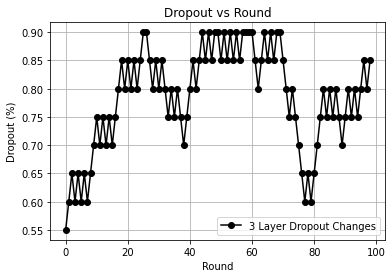
\includegraphics[width = .5\linewidth, height = .4\linewidth]{img/Drop_Round.png}
\caption{Change in dropout rate throughout the training process.}
  \label{fig:drop}
\end{figure*}

\textbf{Model: }We use a CNN model consisting of one $(3 \times 3)$ convolution layer, followed by a one max-pool and several fully connected layers. We use softmax as an activation in the final layer. For Cifar data sets we use an input size of $(32 \times 32 \times 3)$. This model has a total of 923k trainable parameters. We use validation accuracy as evaluation method. We use TensorFlow for implementation of the models.

\textbf{Hyper-parameters: } We have used Adam optimizer with sparse categorical cross-entropy as loss function. We use the known baseline settings of FedAvg without any changes. Our federated learning experiments are performed with 10 clinets running simultaneouly using the Flower framework.

\begin{figure*}
  \centering
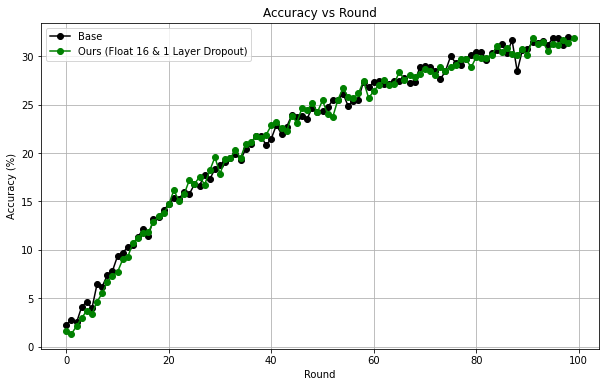
\includegraphics[width = .5\linewidth, height = .4\linewidth]{img/Acc_Cifar100.png}
\caption{Accuracy of our method compared with base FedAvg on Cifar100. The plot shows that our validation accuracy is better the base case.}
  \label{fig:cifar100}
\end{figure*}

\textbf{Quantization: } Our quantization is inspired by previous work of Jacob et al \cite{jacob2018quantization}. We use 'float16' quantization which is able to achieve 2x compression with minimal accuracy loss. We apply quantization at the end of each client round.

\textbf{Adaptive federated dropout: } For base case our model doesn't have any dropout. We compare this with adaptive dropout applied after 1 fully connected layer and applied after 3 fully connected layers. We only experiment with applying dropout on fully-connected layers, since CNN layers have very few parameters. Our adaptive federated dropout has two more hyper-parameters $\alpha$ and $\beta$. We start with a dropout rate of .5 and use .05 as value of $\beta$, .1 as value of $\alpha$. That means we increase or decrease the dropout rate by .05, unless it's equal to .9 or .1. We plot the changes in dropout rate throughout the training process in Figure \ref{fig:drop}.

\begin{figure*}
  \centering
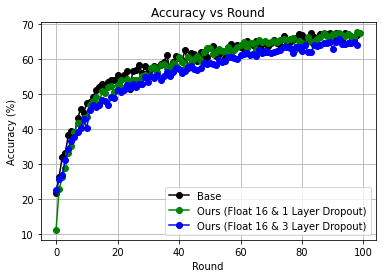
\includegraphics[width = .5\linewidth, height = .4\linewidth]{img/Acc_Cifar10.png}
\caption{Accuracy of our method compared with base FedAvg on Cifar10. The plot shows that our validation accuracy is very similar to the base case even when we remove significant amount of parameters with dropout and quantization.}
  \label{fig:fed_cifar}
\end{figure*}

\begin{figure*}
  \centering
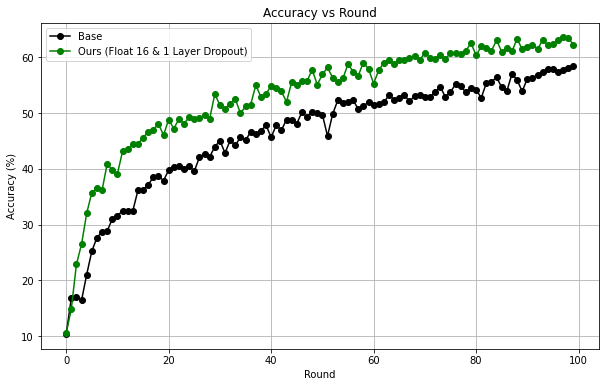
\includegraphics[width = .5\linewidth, height = .4\linewidth]{img/Acc_Cifar10_Imb.png}
\caption{Accuracy of our method compared with base FedAvg on Imbalanced Cifar10. The plot shows that our provides advantage over FedAvg in case of class imbalance while significantly reducing communication needs.}
  \label{fig:imb_cifar}
\end{figure*}


We plot the results of Cifar 10 data set with 'float16' quantization (2x compression) and different amount of dropout in Figure \ref{fig:fed_cifar}. A dropout in one layer combined with quantization leads to approximately 3x reduction in communicated parameter size and a 3 layers of dropout with quantization leads to approximately 4x reduction in parameter size. The results for Cifar100, presented in Figure \ref{fig:cifar100} show that our method achieves similar results accross different data sets.


\textbf{Robustness to class Imbalance: }To test the robustness to imbalanced data we use imbalanced Cifar10 with the number of samples for class 0 and 1 reduced by half. We plot the results of imbalanced cifar10 in Figure \ref{fig:imb_cifar}. The results show that our method provides advantage over FedAvg in case of imbalanced data set. The dropout rate increase in clients with more data from majority classes and works as a regularization.

\textbf{Limitations}
Our study assumes that all node devices involved in the federated learning network are capable of meeting the computational requirements necessary for efficient algorithm performance. This assumption might not accurately reflect the varied capabilities of devices in practical, real-world applications and could skew the model's performance metrics. To counteract the risk of over-fitting, we have employed multiple datasets, namely datasets Cifar10 and Cifar100. Utilizing multiple datasets helps to verify that our model's efficacy is generalizable and not overly tailored to specific data characteristics. Using quantization would lead to some loss of precision and that might introduce domain adaptation problem in some cases. 

\section{Conclusion}

Federated learning is dependent on client device performance and communication bandwidth. Both of these can vary a lot based on different demographic groups and thereby exclude people from training models. Research on dropout and quantization methods can address this problem and improve the application of federated learning. Our work can lead to massive reduction in communication overheads while still being robust to class imbalance issue. To address these issues more, in future we plan to work on client sampling and investigate the use of heterogeneous models in federated learning.

% The images, the method section and results still need a lot of work. we plan to test 4 bit/8 bit quatization and hopefully add that. We can run more experiments with different data sets , different values of alpha, beta and different number of clients.

% Typical review feedback in federated learning papaers are these : 

%Violates the privacy preserving feature of FL : Does not in our case
%Computational burden : Quantization
%Novelty and related work section is not satisfactory : Our method is novel
%Quality of the presentation : We can improve this
%Missing comparison against popular baselines : We plan to compare with other federated dropout method, pruning method and a few other papers listed below : 
%https://flower.ai/docs/baselines/dasha.html
%https://flower.ai/docs/baselines/niid_bench.html
%https://flower.ai/docs/baselines/fedmlb.html
%https://flower.ai/docs/baselines/tamuna.html

\bibliographystyle{splncs04}
\bibliography{main}
\end{document}